\chapter{Literature Review}
\label{chp:LitReview}
This chapter aims to describe the context within which the project is undertaken. The purpose of this literature review is to accumulate a thorough understanding of the current state of technology relevant to the project. Attention will be given to technical theory and work done by others in this field of research.

\medskip

An overview will be given about the anatomy of the ear which is relevant to this study. Next, background will be given about each vital sign. Thereafter, the current technology available for monitoring vital signs will be reviewed.

\section{Ear Anatomy} %----------------------------------------------------------------------------------
The area of the ear that is relevant to this study is the external ear. It includes the auricle, ear canal with surrounding tissue and the lateral side of the tympanum. This is the area available for the Ear-Monitor to take the bio-signal measurements. Each part of the ear anatomy will be described, especially with regards to its ability to emit bio-signals or support the device in another way.

\subsection{Auricle}
The auricle is the visible part of the ear. It forms a C-shaped funnel that protrudes from the scull. Its structure is predominantly formed by yellow elastic cartilage covered in skin. Its complex folded shape differs from person to person, but certain structures are present in all normal auricles and have been named. As can be seen on Figure~\ref{fig:AuricleLabel} the concha is the indented part next to the ear canal. This area is an ideal location for a wearable device. The device can be held in place by the tragus and a probe can easily extend into the ear canal.

\medskip

The external ear is supplied with blood from the auricular arteries. These arteries branch from the carotid artery which supplies the rest of the brain with blood. Being made mostly of cartilage and being at an extremity of the body, the auricle is not a suitable location for taking temperature measurements for its temperature is easily influenced by the ambient conditions.

\medskip

\begin{figure}
   \centering
   \includegraphics[scale=1]{figs/AuricleLabel}
   \caption{Drawing of the auricle (Get source from: goo.gl/mmLnFx)}
   \label{fig:AuricleLabel}
\end{figure}

The layer of skin covering the auricle contains blood vessels. It is possible to detect a pulse in the auricle, in fact, the ear lobe is a popular location for traditional pulse oximetry measurements. This is a possible location for a ear-worn device to make a heart rate measurement \citep{poh2010motion}. The ear lobe's blood vessels are, however, susceptible to vasoconstriction due to cold or hypovolaemia \citep{WHO2011UsingPulseOxi}. This will reduce the blood perfusion of the subcutaneous tissue making it harder to get accurate heart rate and blood oxygen saturation measurements.

\medskip

The auricle is used in EEG systems as a location for a reference electrode. It is far enough from the brain for it to have an extremely small electrical potential \citep{nunez2006electric}.

\subsection{Ear Canal}
The external ear canal is the tube running from the floor of the auricle to the middle ear, ending blindly at the tympanic membrane or tympanum. Figure~\ref{fig:EarSection} depicts the structure of the ear as seen from a coronal plane section. The auricle is visible and the shape and relative size of the canal can be observed.

\medskip

\begin{figure}
   \centering
   \includegraphics[scale=0.7]{figs/EarSection}
   \caption{Structure of the ear (Drake et al: Gray's Anatomy for Students)}
   \label{fig:EarSection}
\end{figure}
 
The ear canal in adults is approximately 25 mm long and have a diameter of 5 to 7 mm \citep{alvord1997anatomy}. The outer third of the external ear canal is surrounded by cartilage and fibrous tissue \citep{ExternalAuditoryCanal}. The inner two thirds are surrounded by the temporal bone. Thin skin from the lining of the canal and contains glands secreting ear wax. Hairs are found in the outer part of the canal. The ear canal of infants starts out relatively straight, but obtains a definite S-shape as the head develops \citep{alvord1997anatomy}. This S-shape is important to keep in mind while placing a sensor to measure tympanic temperature. Ear canal size also varies from person to person. Therefore, an ear probe should be designed to fit in a variety of in ear canal shapes and sizes.

\medskip

The secluded nature of the ear canal means that it has a relative constant temperature. Air trapped in the canal by a plug of high thermal resistance will reach thermal equilibrium close to the temperature of the canal wall and tympanum. This is a better location for a core temperature measurement, but will still be influenced by the ambient temperature.

\medskip

The wall of the ear canal is well supplied with blood. Blood vessels just beneath the thin layer of skin makes the ear canal a possible location for measuring heart rate and blood oxygen saturation. The still nature of the head will minimize movement artefacts.

\medskip

The ear canal extend toward the brain and electrical brain activity is present due to the conductive nature of the tissue. According to \cite{nunez2006electric} currents from brain potentials can be focused through holes in the scull, like the ear and nose. The farther away the origin of the signal is from the electrode, the weaker the measured signal will be. Therefore, an electrode in the ear canal will detect electrical brain activity near the ear better, including the temporal lobe and brain stem.

\subsection{Tympanum}
The tympanum forms the medial boundary of the external ear canal. It is a smooth elliptical membrane with a thickness of about 0.074 mm \citep{alvord1997anatomy}. The membrane is slanted with regards to the external ear canal.

\medskip

As with the rest of the external ear, the tympanum is supplied with blood from a branch of the carotid artery, therefore sharing its supply with the brain including the hypothalamus, the thermoregulation centre of the body. It is the most medial part of the external ear, and is therefore the least susceptible to influence by the ambient temperature. This is the reason that the tympanum is one of the best locations to measure core body temperature. The location is used by physicians to measure core temperature for it is quick and minimally invasive. Variations in body temp can be sensed faster on the tympanic membrane than on other locations on the body. Contact with the tympanum can cause discomfort and harm to the patient, so non-contact infra-red thermometers are usually used.


\section{Medical Sign Physiology} %----------------------------------------------------------------------------------
This section reviews the theory and research done about the physiological aspects of each medical sign that the Ear-Monitor is required to measure. The importance of each of the five medical sign will be discussed, as well as the bio-signals that are used to detect them. This includes the typical range of measurements expected from healthy adults, as well as the causes and implications of deviations from these healthy measurements.

\subsection{Core Temperature}
Thermoregulation is the body's way of keeping its internal temperature within certain bounds to create a favourable environment for chemical reactions to take place. The temperature control centre of the body is in the hypothalamus and it regulates temperature by maintaining a fine balance between heat production and heat loss. Normal human core temperature varies between $36.5^{\circ}C$ and $37.5^{\circ}C$ \citep{jones2010biomedical}. Inability to maintain this balance may indicate problems in the well-being of a person. Elevated temperature (hyperthermia) due to a fever can indicate the presents of an infectious disease. Abnormally low temperature (hypothermia) can be caused by cold exposure, metabolic disorders or infection. Both hyper- and hypothermia can be life threatening. A core temperature measurement is often a key indication to start a treatment or not. Therefore, temperature measurement is part of a full clinical examination and part of the vital sings group of medical signs.

\medskip

The location where temperature is measured is a key factor, for temperature is not constant throughout the body. This is because heat production and heat loss are not constant throughout the body, meaning extremities are usually cooler than the core. Traditional locations for measuring temperature are the tympanic membrane, axilla, mouth, rectum, oesophagus, forehead and urinary bladder. The mean temperature of these areas varies as well. A systematic literature review done by \cite{sund2002normal} combined the results of 20 studies to identify oral, rectal, tympanic and axillary temperature ranges in healthy humans. Table~\ref{fig:VariationsInTemp} shows the results.

 \begin{figure}
   \centering
   \includegraphics[scale=0.3]{figs/VariationsInTemp}
   \caption{The results from 20 studies with strong or fairly strong evidence of normal oral, rectal and tympanic temperature ($^{\circ}$C) in adult men and women are presented. Temperature is obtainable as mean value(bold lines), 1st and 3rd quartiles (unfilled bars) and range (thin lines).}
   \label{fig:VariationsInTemp}
\end{figure}

Studies have also been done comparing measurements at distinct locations to pulmonary artery temperature in ill patients. A study has shown ear-based  $0.07\pm 0.41$  $^{\circ}C$; urinary bladder  $0.03\pm 0.23^{\circ}C$; oral  $0.05\pm 0.26^{\circ}C$; and axillary $-0.68\pm 0.57 ^{\circ}C$. The accuracy of each method varied with the level of pulmonary artery temperature. Repeated measurements with all four methods had mean standard deviation values within $\pm 0.2^{\circ}C$ \citep{erickson1993comparison}.

\medskip

A second study done by \cite{lefrant2003temperature} showed the following results: oesophageal  $0.11 \pm 0.30^{\circ}C$, rectal $-0.07 \pm 0.40^{\circ}C$, axillary $0.27\pm 0.45^{\circ}C$, inguinal $0.17 \pm 0.48^{\circ}C$, urinary bladder $-0.21 \pm 0.20^{\circ}C$.

\medskip

The location of the device in development is restricted to the ear, therefore the tympanic membrane is the preferred location to take temperature measurements. The referenced studies show that the tympanic membrane is a valid location to measure accurate core temperature.

\subsection{Heart Rate}
The presence of a heart beat is paramount to sustain the vital cardiac output, supplying blood to the whole body. Heart rate can be controlled or maintained through two different regulatory systems: The intrinsic conduction system and the nervous system. The intrinsic conduction system works through the rhythmic contraction and relaxation of the heart muscle tissue. The heart rhythm is regulated by the sinoatrial node. The nervous system can influence the heart rate through sympathetic and parasympathetic nerves running from the cardiovascular centres in the medulla oblongata to the heart. The heart beat rate is varied to control the blood flow and blood pressure in the body.

\medskip

The heart is the source of a group of bio-signals. The firing of nodes and propagation of electrical charges through neurons and the conductive cardiac muscle gives of an electrical signals that can be detected. The contraction of the  ventricles forces blood into the arteries, causing a temporary increase in blood pressure. This pressure increase propagates though the arteries as a wave, causing a temporary local increase on blood volume. Pressure- and volume changes can be detected. Blood turbulence and the opening and closing of heart valves causes the characteristic heart sound and chest movements, both sources of bio-signals.

\medskip

Heart rate is influenced by numerous physiological factors including $O_2$, $CO_2$, $H^+$ levels, blood pressure, stress and exercise. Pathological factors can include fever, sepsis, heart disease and anaemia. Tachycardia is abnormally high resting heart rate, generally above 100 bpm, whereas bradycardia is a lower than normal resting heart rate, usually below 60 bpm \citep{normalRestingHR}. Although these two conditions are not necessarily danger signs, it may be an indication of health problems and therefore heart rate measurement is part of any medical examination and one of the vital signs group of bio-signals.

\subsection{Respiratory Rate}
Respiration is the first step in the chain of events to get oxygen to the body's cells for metabolism to provide the body with energy. Respiration ventilates the lungs with air through inhalation and exhalation. The respiratory rate of a healthy adult at rest is usually between 12 and 20 breaths per minute \citep{medscapeBreathingRate}. This can vary drastically if the body is experiencing physical or emotional stress. In increase in respiratory rate can be cause by a fever, pulmonary dysfunction or any one of numerous medical conditions. Respiratory rate is also part of the vital signs group of bio-signals.

\medskip

Respiratory rate monitoring is especially useful for diagnosing sleep apnoea. Symptoms include regular pauses in respiration or periods of shallow breathing (hypopnea) during sleep. This causes an oxygen deficiency in the body and lowers the quality of sleep. Short term symptoms include excessive daytime sleepiness, morning headaches, impaired alertness, and vision problems. If left untreated sleep apnoea can lead to high blood pressure, diabetes, depression, worsening of ADHD, stroke, heart failure, irregular heartbeats, and heart attacks \citep{webMDSleepApnoea}. Sufferers may be unaware of their condition and a sure-fire method of diagnosing it is my monitoring respirator rate during sleep, traditionally done during an overnight sleep study.

\subsection{Blood Oxygen Saturation}

Haemoglobin is the oxygen transporter protein found in the red blood cells of blood. Blood gets oxygenated in the lungs and then carries $O_2$ to the rest of the body for aerobic respiration necessary to produce energy. The correct levels of oxygen in the blood is vital to the health of the individual.

\medskip

Oxygen saturation, $SO_2$, refers to the concentration fraction of oxygenated haemoglobin to total concentration of haemoglobin in the blood:

$$SO_2  =  \frac{C(HbO_2)}{C(HbO_2)+C(Hb)}$$

Where $C(HbO_2)$ is the concentration of deoxygenated haemoglobin (deoxyhaemoglobin) and $C(Hb)$ is the concentration of oxygenated haemoglobin (oxyhaemoglobin).

\medskip

Blood oxygen saturation of 95-100\% is normal in healthy humans. Hypoxaemia is the condition when the saturation is below 90\%. This can be an indication of circulatory or ventilatory problems, anaemia or sleep apnoea. Levels below 80\% can hinder organ function and can lead to organ failure and cardiac- or respiratory arrest. The brain in extremely susceptible to damage due to a lack of oxygen. Cerebral hypoxia is the insufficient supply of oxygen to the brain. This can cause brain damage and in severe cases, brain death.

\subsection{Electrical Brain Activity}
EEG, or electroencephalography, is the recording of the electrical activity in the brain. The neurons in the brain



\section{Bio-signals Measurement Theory} %-----------------------------------------------------------------------------
This section will focus on the theory and current technology relevant to the measurement of each medical sign required of the Ear-Monitor. Attention will be given to the different bio-signals available to determine each medical sign and the different methods of transducing and measuring these bio-signals. This section will also make reference to various articles and studies done by other researchers in this field of study. The aim is to gather all the relevant information in order to make an informed selection of the methods and sensors the Ear-Monitor will use to measure each medical sign.

\subsection{Core Temperature}
Various methods are available for measuring core temperature. Non-electric, fluid-filled thermometers was the first to be used. The mercury-filled thermometer was used by early physicians to study the thermoregulation of the human body and crudely identify fevers. Since then, the mercury has been replaced by coloured alcohol or another heat sensitive liquid, due to toxicity of mercury.

\medskip

Another type of fluid-filled thermometer is the liquid-crystal thermometer. It contains liquid crystals that changes colour when at different temperatures. The use of these two types of fluid-filled thermometers has decreased significantly due to the accuracy, speed and connivance of digital thermometers.

\medskip

Electrical thermometers are now the industry standard of measuring core temperature. Central to any digital thermometer lies a transducer that convert temperature to an electrical signal. Resistance temperature detectors, thermocouples thermistor and thermopiles will be discussed. They can be divided into contact and non-contact thermometers.

\subsubsection{Contact Thermometers}
These are a family of thermometers that measure their own temperature with the assumption they and the object whose temperature are of interest are in thermal equilibrium. Therefore, they are usually placed in contact with the object. When using a contact thermometer n the ear, the sensor part of the thermometer can be placed in contact with the ear canal wall, the air inside the canal or with the tympanic membrane self.

\subsubsection{Resistance Temperature Detector}

Resistance temperature detectors (RTDs) uses the temperature-resistance relationship for metals to measure temperature. Thin wire coils or films of platinum, copper or nickel are usually preferred for they have a stable and repeatable temperature-resistance relationship over a large temperature range.

\subsubsection{Thermocouple}
Thermocouples make use of the thermo-electric effect to make a temperature measurement. They consist of two dissimilar conductors connected at the one end, knows as the hot junction (measuring junction). The other ends of the two wires are known as the cold junction (reference junction) and are connected to a voltage meter via common conductors. A voltage is generated dependant to the temperature difference between the measuring- and reference junctions. Thermocouples do not respond to absolute temperature; therefore, their accuracy depends on how well the reference temperature can be defined. Reference temperatures are usually determined by a precise thermistor. Thermocouples are very versatile and widely used in clinical applications, but the downsides are that their output signal is low and non-linear, therefore requiring a sensitive and stable voltage measuring device \citep{jones2010biomedical}.

\medskip

Thermocouples can be connected in series and are then called thermopiles. This configuration sums the output voltages, resulting in temperature averaging. This method improves accuracy by reducing noise. 

\subsubsection{Thermistor}
A thermistor is a type of semiconductor whose resistance varies with changes in temperature. They differ from RTDs in that they are usually made of ceramics, they have higher precision over a smaller temperature range and they can have a negative relation to temperature. Thermistors are preferred above RTDs and thermocouples for use as biomedical sensors due to their faster response time and higher sensitivity over a smaller range and. The smaller range does not matter, for the temperature range of interest in biosensors are small and well defined. 

\subsubsection{Application}
In the case of RTDs and thermistors, the measuring element is placed in position and a current is sent through the sensor. By measuring the voltage across the resistive element, it is possibly to calculate the voltage and subsequently determine the temperature. In the case of the thermocouple, the hot junction can be placed in contact with the canal wall or tympanum. Typically, the hot junction will be enclosed with a soft material to protect the canal and tympanum. The canal is sealed off and time is allowed for the area to equilibrate to tympanic temperature. Commercial devices like Novatemp\textsuperscript \textregistered and Starboard\textsuperscript \textregistered claims a $\pm$ 0.2 $^{\circ}C$ accuracy.

\medskip

Placing a thermometer in contact with the tympanic membrane will give an accurate measurement, but can cause discomfort to the wearer. There is also a risk of harming the tympanic membrane. Sensors in contact with the ear canal wall or the air inside the canal run the risk of making errors by measuring the temperature of objects that are not in thermal equilibrium with the tympanic membrane. Therefore, non-contact thermometers will be considered.

\subsection{Non-contact Thermometers}
Thermopiles can be used to detect thermal radiation without being I contact with the object. All matter with temperatures above 0 K radiates electromagnetic radiation according to the Stefan-Boltzman law. The thermal radiation, $Q$, per unit area is given by the equation:

$$Q=\varepsilon \sigma T^4.$$

Where $\varepsilon$ is the emissivity, $\sigma$ the Stefan-Boltzman constant and T the temperature of the object.

The wavelength distribution varies according to the temperature of the object and is described by Planck's law:

$$B_\lambda (\lambda ,T)=\frac{2hc^2}{\lambda ^5}\frac{1}{e^\frac{hc}{\lambda k_B T} -1}.$$
 
Where $B_\lambda$ is the spectral radiance, $\lambda$ the radiation wavelength, $h$ Planck's constant, $k_B$ Boltzman's constant $c$ the speed of light and $T$ the object's temperature. Through maximizing $B_\lambda$ , it is possible to find the dominant wavelength that is emitted at a certain temperature. Figure~\ref{fig:PlancksLaw} shows a plot made of spectral radiance versus wavelength at $T=$ 37 $^{\circ}C$, the core temperature of humans. It can be seen that the dominant wavelength is at 9.35 $\mu$m. This is in the infrared range, and therefore this type of thermal radiation thermometer is called an infrared thermometer.

 \begin{figure}[h]
   \centering
   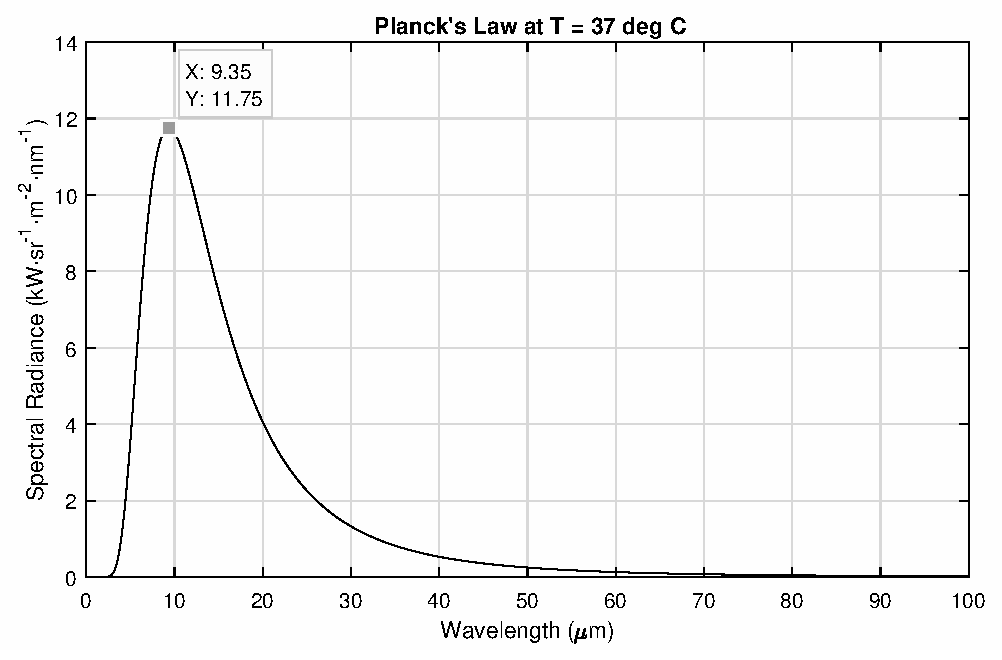
\includegraphics[scale=0.6]{figs/PlancksLaw}
   \caption{Plot showing how Planck's law can be used to determine the dominant radiation wavelength at certain temperature}
   \label{fig:PlancksLaw}
\end{figure}

In the case of measuring the temperature of the tympanic membrane, the hot junction's temperature will be determined by the radiation received from the tympanum minus the radiation radiated by the sensor self.

\medskip

When talking about thermal radiation, an important aspect is emissivity. Emissivity is the ability of an object to radiate thermal energy. It is quantified as a ratio of thermal energy emitted by a surface relative to the thermal energy emitted by an ideal black body at the same temperature. A black body is an idealized surface that reflects no radiation, meaning all energy radiated from the surface are due to the temperature of the surface. Thus, a black body have an emissivity of 1 and have the maximum theoretical radiation at a given temperature. The accuracy of an infrared sensor depends on the ability of the object to emit sufficient thermal radiation for the sensor to detect. Cross-referencing various emissivity tables, it was found that the emissivity of human skin is 0.98, meaning that it is an excellent emitter of thermal energy \citep{stumme2003emissivity} \citep{EmissivityThermoWorks} \citep{EmissivityOptotherm}. The ear drum is covered with skin, making it an ideal target object for a non-contact thermometer.

\medskip

An infrared thermometer generally consists out of a thermophile attached to a blackbody and shielded by an infrared filter that also acts as a lens to focus infrared waves \citep{irTempSensors}. This setup, shows in Figure \ref{fig:IR_Thermometer}, allows for the non-contact temperature sensing of the tympanic membrane. Unlike pulse rate, breathing and electrical brain activity, the core body temperature varies slowly. It takes minutes to vary significantly. Therefore, the sampling period of core temperature can be as long as 10 seconds.

\medskip

\begin{figure}[h]
   \centering
   \includegraphics[scale=0.5]{figs/IR_Thermometer}
   \caption{IR Thermometer diagram (V Polyzoev et al: Demystifying Thermopile IR Temp Sensors)}
   \label{fig:IR_Thermometer}
\end{figure}

\subsection{Commercial Devices}
The \textit{degree}$^{\circ}$, Figure \ref{fig:Degree}, is a continuous in-ear thermometer for children, developed by \textit{cosinuss}$^{\circ}$, a company specialising in wearable sensors. The bulk of the device is worn behind the ear, and there is a wire running over the auricle to the ear canal, in which a probe is placed. The device takes its temperature measurements with a sensor placed in contact with the canal wall. The manufacturer claims an accuracy of $\pm$0.1 $^{\circ}C$. It monitors temperature continuously and sends real time data to a mobile phone.

\medskip

\begin{figure}
   \centering
   \includegraphics[scale=0.65]{figs/Degree}
   \caption{CAD model of the \textit{degree}$^{\circ}$ from the \textit{cosinuss}$^{\circ}$ website (include ref)}
   \label{fig:Degree}
\end{figure}

Apart from the \textit{degree}$^{\circ}$, there are not much literature on wearable ear thermometers. Two patents were found describing similar devices: US 6556852 B1 and US 20090221888 A1. The first of which proposes the use of an infrared sensor pointed at the tympanic membrane, and the latter not specifying the method of measuring. Hopefully, the tests planned for this study can add to this insufficient body of knowledge.

\subsection{Heart Rate}
The presence of a heart beat is a paramount to the sustain the vital cardiac output supplying blood to the whole body. Heart  rate can be controlled or maintained through two different regulatory systems: The intrinsic conduction system and the nervous system. The intrinsic conduction system works through the rhythmic contraction and relaxation of the heart muscle tissue. The heart rhythm is regulated by the sinoatrial node. The nervous system can influence the heart rate through sympathetic and parasympathetic nerves running from the cardiovascular centres in the medulla oblongata to the heart. The heart beat rate is varied to control the blood flow and blood pressure in the body.

Heart rate is influenced by numerous physiological factors including $O_2$, $CO_2$, $H^+$ levels, blood pressure, stress and exercise. Pathological factors can include fever, sepsis, heart disease and anaemia. Tachycardia is abnormally high resting heart rate, generally above 100 bpm, whereas bradycardia is an lower then normal resting heart rate, usually below 60 bpm. Although these two conditions are not necessarily danger signs, it may be an indication of health problems and therefore heart rate measurement is part of any medical examination and one of the vital signs in humans.

Heart rate can be measured in a variety of ways. Electronic ways of measuring heart rate include electrocardiography (ECG), photoplethysmography (PPG), ballistocardiography(BCG), electronic stethoscopes and Doppler flow-meters.

\subsubsection{Electrocardiography}
ECG records the electrical activity of the heart over a period of time. It is the the recommended way of monitoring heart rate in most intensive care units. A cardiologist will use a 12 lead ECG with 10 electrodes placed in a specific configuration on the chest. Various wearible devices use ECG to measure heart rate. Fitness monitors normally uses a chest strap with electrodes to detect the heart's electrical activity. Studies have been done developing wearable ECGs for clinical use.

The typical telemedicine set-up of a wearable ECG is a signal acquisition module, collecting and sending data by means of a wireless transceiver to a smart-phone, which then uploads the data to a healthcare server \citep{wang2010wearable} and/or \citep{prawiro2016integrated}. %Maybe put this paragraph in a design related chapter

The latest in wearable ECK systems is the use of Dry Polymer-based electrodes \citep{wang2010wearable} or non-contact electrodes that can be place on top of clouthing \citep{lin2013development}. This is an improvement above the standard conductive gels or adhesives and can be used repeatedly. But these electrods still needs to be place on the chest. An ear located ECG monitor have been developed by \cite{winokur2012wearable}. This device uses an one lead set-up with on electrode place on the mastoid bone and one on the neck. This configuration relies on the conductive properties of human tissue to carry electrical charges form the heart to the location of the ear. (See also: Bluetooth Low Energy (BLE) Based Mobile Electrocardiogram Monitoring System; 

\subsubsection{Photoplethysmography}
Photoplethysmography (PPG) is an optically obtained  plethysmogram (volume change of an organ). PPG can be used to measure the change in volume of blood vessels close to the skin surface. When the left ventricle contracts a pressure pulse propagates through the arteries from the heart to the extremities of the body. This wave corresponds to the systolic blood pressure. Blood vessels walls contain elastic fibres that allow them to stretch. This means that the diameter of vessels will increase when the blood pressure increase, causing   arteries so to stretch and contract with each heartbeat. A PPG can be used to measure this variation.

According to Lambert's law, the amount of light absorbed is proportional to the length of the path that the light has to travel in the absorbing substance. Therefore a change in blood vessel diameter will cause a change in tissue absorption. Light shined through the skin to illuminate the underlying subcutaneous tissue can either be reflected, absorbed or allowed to transmit through the tissue. Changes in the light absorption of the tissue can be detected by measuring this reflected or transmitted light. As defined by Lambert's law: changes in absorbed light is due to the changes in arterial diameter and thus, an indication of the pulse. Figure of reflective and transmittance PPG.

A photoplethysmogram of blood vessels is obtained through pulse oximetry. A pulse oximeter consiste of a light emitter and detector. It can operate in reflectance or transmittance modes as shown in Figure~\ref{fig:PulseOxiModes}. Transmittance pulse oximetry measures the light that is allowed to transmit through the tissue. It is more common, but its placement is restricted to a thin part of the patient's body that will allow light through. Reflectance pulse oximetry has no such restrictions for it measures the light that is reflected by the tissue.

\begin{figure}
   \centering
   \includegraphics[scale=1]{figs/PulseOxiModes}
   \caption{Pulse oximetry in reflective or transmittance modes}
   \label{fig:PulseOxiModes}
\end{figure}

The signal read by the photo detector of the pulse oximeter consists of a AC component superimposed on a DC signal. The DC component is the constant reflection of light by the body's tissue: skin, fat, venous blood and the non-pulsating arterial blood. The AC components is the variation in reflected light due to the change in diameter of the arteries and is usually between 0.5 - 2\% of the DC component  \citep{tavakoli2006analog}. Therefore the frequency of the AC component is synchronised to the heart rate.

\subsubsection{Ballistocardiography}
Ballistocardiography (BCG), also known as a seismocardiogram, is the measurement of the mechanical effects of the beating heart. Typically accelerometers or pressure sensors will be used to measure movement or forces on the surface of the body. BCG has been researched for use in ear heart rate extraction. In a wearable device proposed by \cite{da2010ear}, mechanical vibrations associated with heart rate are converted to electronic signals through capacitive sensing electrodes. This method works my measuring the change in capacitance between the two electrods as the distance between them changes due to heart rate vibrations. A study by \cite{winokur2012wearable} proposed measuring the head-to-foot axis recoil during the principal blood-volume shift during cardiac ejection. This is done by placing an MEMS accelerometer behind the auricle. Due to the movement dependent method of operation this technology is extremely susceptible to motion artefacts and it can only be used during which the body is stationary.


The traditional and simplest of which is placing an index and middle finger on the wrist and counting the arterial pulses felt per minute. In fact, heart rate pulse can be felt throughout the body where large arteries are close to the skin.

A variation of this technology is discussed in a article by \cite{park2015wearable}. They propose using a scissor shaped hinge mechanism in the ear canal that measures the change in the canal size due to the in-ear blood pulse waves. The mechanical movement it converted to an electrical signal through a piezoelectric film sensor.

\subsubsection{Other methods}
Electronic stethoscopes uses an microphone to record heart sounds. The hears makes a distinct series of sounds during the cardiac cycle due to blood turbulence and the shutting of heart valves. The period of this sound series can be used to determine heart rate and does not require skin-contact.

A Doppler flow-meter can be used to detect the alternating blood current component in near-surface arteries. This component is synchronised to the heart rate frequency. The device can use ultrasound, microwaves of light to achieve the Doppler shift.

\subsection{Respiratory rate}
Breathing is a process critical for life. Respiration is the first step in the chain of events to get oxygen to the body's cells for metabolism to provide the body with energy. Breathing and plus it the first signs of life to check for in a medical emergency. %Say this better

How is the RR controlled

Appart form the obvious face that a lack of breathing is a problem, the RR can divulge some information about a persons health. What does the RR tell us about health


Measure through baseline oscillations of BCG signal (see The Ear as a Location for Wearable Vital Signs Monitoring \citep{da2010ear})

Respiratory rate is the rate at which ventilation takes place in the lunge. One inhalation and exhalation cycle is counted a breath and respiratory rate is usually measured in breaths per minute. Healthy adults have an resting respiratory rate of between 12 and 18 breaths per minute., This can vary drastically if a the body is experiencing physical or emotional stress.

It is important to monitor breathing, for irregular breathing or difficulty to breathing may be an induction of healthy problems. Apnoea is when breathing stops completely. This is especially an danger in infants and patients in the ICU.

Traditionally, respiratory rate is measured by counting the number of timer the chest visibly rises as a person inhales. Other methods include listening to the chest with a stethoscope and counting audible breaths, fixing an accelerometer to the chest, measuring CO\textsubscript{2} levels in the respiratory gases and looking at variations in heart rate.

Caretakers are usually very concerned about sleep apnoea in infants, as cause a risk for infant mortality. Apnoea monitors are available to warn caretakers if breathing halts. These monitors usually measure force or acceleration caused by the breathing of the sleeping infant. The device can be worn by the infant or can by placed in the cot.


All respiratory related measurements in the reviewed products rely on movement sensors attached to the body of the infant that senses its movement. Sensors include accelerometers and the \textit{BreathOptic}\textsuperscript{\texttrademark} sensor used by Sleep-Mat. These sensors detect the chest movement produced by the infant while breathing. In some cases, like Mimo and Sleep-Mat, these sensors are sensitive enough to determine the infant's respiratory rate from this movement. In other products, such as Anglecare and Monbaby, the sensors are sensitive enough to register the movement due to breathing, but not sensitive enough the extract the rate of breathing.
Alerts are sent wirelessly to the cellphone of the caretaker if the movement stops for a certain amount of time. This may indicate that the infant has stopped breathing. The problem with this method is that products like Monbaby, Anglecare and Mimo will only alert the caretakers once the infant has stopped breathing completely for 15 or 20 seconds. This may be too late to prevent an infant mortality. A product is needed that can accurately monitor the respiratory rate and warn the doctor or caretakers if the respiratory rate drops or becomes irregular.
Respiratory sinus arrhythmia (RSA) is the baseline oscillation in heart rate in synchrony with the respiratory rate. It is observed as an increase in heartrate during inspiration and a decrease during expiration. According to a study done by Stratton JR et al, the variation in heart rate due to RSA is higher in younger test subjects with 74\% increase in children vs. 52\% increase in adults [5]. These findings support the use of RSA to determine the infant's respiratory rate. A study has been done by D da He investigating the use of ballistocardiogram heart rate measurements to detect RSA [6]. This project will attempt to detect RSA in pulse oximetry heart rate measurements. This is a unique approach in wearable monitoring devices. The advantage is that no extra sensors, like accelerometers, are needed for the measurement of respiratory rate.

\subsection{Blood Oxygen Saturation}
Haemoglobin is the oxygen transporter protein found in the red blood cells of blood. Blood gets oxygenated in the lungs and then carries \(O_2\) to the rest of the body for aerobic respiration necessary to produce energy. The correct levels of oxygen in the blood is vital to the health of the individual.

Oxygen saturation ($SO_2$) refers to the fraction of oxygenated haemoglobin to total haemoglobin in the blood: $$ SO_2 = \frac{C(HbO_2)}{C(HbO_2)+C(Hb)}\times100\% $$ Where $ C(HbO_2) $ is the concentration of deoxygenated haemoglobin (deoxyhaemoglobin) and $ C(Hb)$ is the concentration of oxygenated haemoglobin (oxyhaemoglobin).

Blood oxygen saturation of 95-100\% is normal in healthy humans. Hypoxemia is the condition when the saturation is below 90\%. This can be an indication of circulatory or ventilatory problems, anaemia or sleep apnoea. Levels below 80\% can hinder organ function and can lead to organ failure, cardiac- or respiratory arrest. In the absence of oxygen, damage to the brain starts within 5 minutes with brain death ensuing within another 10 to 15 minutes.

Oxygen saturation can be measured by means of an arterial blood gas test resulting an arterial oxygen saturation reading. An alternative method is pulse oximetry. This method measures peripheral capillary oxygen saturation (Sp02). This is a clinically excepted estimation of the arterial oxygen saturation.

Various devices are available for measuring blood oxygen saturation. Elaborate...

\subsubsection{Oxygen Saturation Measurement Theory}
Blood oxygen saturation calculation through pulse oximetry relies on the different adsorption spectra of oxyhaemoglobi) and deoxyhaemoglobin. Figure~\ref{fig:AbsorptionSpectra} shows the absorption spectra of oxy- and deoxyhaemoglobin. It can be noted that deoxyhaemoglobin has a significantly higher absorption of red light (600 - 750 nm wavelength) while oxyhaemoglobin has a slightly higher absorption of infrared light (850 - 1000 nm wavelength). This explains the fact that oxyginated blood apperas bright red and deoxygineted blood is a darker shade of red. (find a source for the image) (What is on y-axis and what is NIR region). Literature usually uses 660 nm (red) and 940 nm (near infrared) http://www.iosrjournals.org/iosr-jeee/Papers/Vol8-issue1/D0812226.pdf?id=7592

\begin{figure}
   \centering
   \includegraphics[scale=0.8]{figs/AbsorptionSpectra}
   \caption{Absorption spectra of oxy- and deoxyhemoglobin}
   \label{fig:AbsorptionSpectra}
\end{figure}

From the Figure~\ref{fig:AbsorptionSpectra} it can be seen that the ratio of absorbed red light to absorbed infra-red light is unique to a certain level of blood oxygen saturation. Therefore this ration can be used to estimate blood oxygen saturation. To account for different DC absorption between patients, a modulated ratio ($R$) is used:
$$R = \frac{\left(\frac{AC}{DC}\right)\textsubscript{red}}{\left(\frac{AC}{DC}\right)\textsubscript{IR}} $$
This ensures that the $ O_2 $ saturation of only the arterial blood is calculated. The ration can be checked against an empirical determined curve. The standard formula for this curve is found in literature as $ \% SpO_2 = 110-25R $, (http://www.ti.com/lit/an/slaa655/slaa655.pdf) but it can vary from device to device. 

\subsection{Respiratory Rate}


\subsection{Respiratory Rate Theory}

\subsection{EEG}

\subsection{EEG Theory}
